\documentclass[11pt]{article}
\usepackage[utf8]{inputenc}
\usepackage{graphicx}
\usepackage{listings}
\usepackage{color}
\usepackage{float}
\usepackage[margin=1in]{geometry}
\usepackage{multirow}
\usepackage{multicol}
\usepackage{todonotes}
\usepackage[toc,page]{appendix}
\usepackage[square,numbers]{natbib}
\usepackage[utf8]{inputenc} % Required for inputting international characters
\usepackage[T1]{fontenc} % Output font encoding for international characters
% \usepackage{mathpazo} % Palatino font

\graphicspath{}

\usepackage{fancyvrb}

\usepackage{markdown}



\newtheorem{theorem}{RQ}

\lstdefinestyle{leftCode}{
  belowcaptionskip=1\baselineskip,
  breaklines=true,
  frame=L,
  xleftmargin=\parindent,
  showstringspaces=false,
  basicstyle=\footnotesize\ttfamily
}


\begin{document}

%----------------------------------------------------------------------------------------
%	TITLE PAGE
%----------------------------------------------------------------------------------------

\begin{titlepage} % Suppresses displaying the page number on the title page and the subsequent page counts as page 1
	\newcommand{\HRule}{\rule{\linewidth}{0.5mm}} % Defines a new command for horizontal lines, change thickness here
	
	\center % Centre everything on the page
	
	%------------------------------------------------
	%	Headings
	%------------------------------------------------
	
	\textsc{\LARGE University of Birmingham}\\[1.5cm] % Main heading such as the name of your university/college
	
	\textsc{\Large Department of Computer Science}\\[0.5cm] % Major heading such as course name
	
	\textsc{\large Dissertation for BSc. Mathematics and Computer Science}\\[0.5cm] % Minor heading such as course title
	
	%------------------------------------------------
	%	Title
	%------------------------------------------------
	
	\HRule\\[0.4cm]
	
	{\huge\bfseries Semantic Analysis of Text}\\[0.4cm] % Title of your document
	
	\HRule\\[1.5cm]
	
	%------------------------------------------------
	%	Author(s)
	%------------------------------------------------
	
	\begin{minipage}{0.4\textwidth}
		\begin{flushleft}
			\large
			\textit{Author}\\
			Tamara \textsc{Herbert} \\
			1557437% Your name
		\end{flushleft}
	\end{minipage}
	~
	\begin{minipage}{0.4\textwidth}
		\begin{flushright}
			\large
			\textit{Supervisor}\\
			Leandro \textsc{Minku} % Supervisor's name
		\end{flushright}
	\end{minipage}
	
	%------------------------------------------------
	%	Date
	%------------------------------------------------
	
	\vfill\vfill\vfill % Position the date 3/4 down the remaining page
	
	{\large April  2019} % Date, change the \today to a set date if you want to be precise
	
	%------------------------------------------------
	%	Logo
	%------------------------------------------------
	
	%\vfill\vfill
	
\includegraphics[width=0.2\textwidth]{litImgs/birmingham.png}\\[1cm] % Include a department/university logo - this will require the graphicx package
	 
	%----------------------------------------------------------------------------------------
	
	\vfill % Push the date up 1/4 of the remaining page
	
\end{titlepage}

%-----------------
\setcounter{tocdepth}{1}
\tableofcontents

\pagebreak
\section{Abstract}

The semantic analysis investigation produced by this project explores structures in which emotions can be represented in a computable format, primarily using a Valence-Arousal-Dominance structure, and optimising sentiment prediction tools using lexicon-based and machine learning methods. Existing semantic analysis tools usually only classify whether input text is positive or negative, and this project aims to explore other ways text can be classified.
Natural Language Processing tools are applied to text-based datasets, and various investigations are carried out to explore the best way to utilise the data for a prediction tool.

This project produces a machine learning model that takes an input sentence and returns Positive/Neutral/Negative classes for the Valence, Arousal and Dominance for the emotion behind the sentence. This model is then applied to a web application that uses this returned data to relate the text to music. 

The findings set out by this project imply that using a more complex structure to represent emotion can lead to a better understanding of input text, and shows that we can apply existing sentiment prediction methods to this structure to obtain an effective model.
\\
\textit{Keywords: Semantic Analysis, Machine Learning, Emotion Prediction, Text Analysis}
\pagebreak

\section{Introduction}

Analysing the emotions behind a piece of text is not always an easy problem even for human readers, and trying to compute this is much harder.

Sentiment analysis of text is a branch of Natural Language Processing where analysis is used to extract and identify subjective information from input data. This style of analytics has wide applications, primarily in marketing and customer service industries where materials such as social media and survey responses are utilised to provide intelligent information about a target market. 

Many sentiment analysis tools that already exist predict whether input text is positive or negative, but very few attempt to obtain more detail about the more complex mood behind it. Understanding something as subjective as an emotion cannot always be put into these discrete binary classes, and as such, exploring whether an emotion can be represented by more than just this one dimension could hold significant value. Applications for establishing a more detailed emotion behind a text could be working out whether a customer who has a complaint about a product is angry or just disappointed, so that appropriate reimbursement can be suggested.

Some existing projects look at how positive a piece of text is in more detail, sometimes ranking sentences on a scale between 1 and 10 but just an emotion over this single dimension is limiting, and exploring whether there is a better way to represent sentiment than this is an interesting topic.
Extensive research has gone into producing sentiment analysis models over a positive-negative dimension with a high level of prediction accuracy, and using the results of these investigations to apply to a more complex emotive prediction model is something that this project aims to examine.

We can formalise this into two main research questions that will be investigated as part of this project:

\subsection{Research Questions}


\begin{itemize}
    \item   \begin{theorem} 
                \label{RQ1}
                \textnormal{How can textual sentiment prediction be optimised?}
            \end{theorem}   
    \item   \begin{theorem} 
                \label{RQ2}
                \textnormal{Is using more than 1 dimension to classify emotions useful?}
            \end{theorem} 
\end{itemize}

After analysis of existing work and exploring what data is available, we can refine these questions further. 

\pagebreak


\section{Sentiment Representation Structures}

\subsection{Ekman's Six Basic Emotions}

There is no universally accepted model for representing sentiments, but a standard for classifying emotions in a categorical model is using Ekmans six basic emotions \cite{Ekman}. These are identified as Anger, Disgust, Fear, Happiness, Sadness and Surprise. Since there are only six discrete classes in which emotions can be placed, this can be argued to be very subjective when classifying \cite{emoBank}, but are very useful in portraying a general result back to user rather than numeric values. Other ways of representing emotion in discrete classes exist, but they are not as popular as Ekman's representation \cite{izard1993stability}.

\subsection{Valence}
A very common way to classify phrases and sentences in sentiment analysis is to analyse the Valence of the text, as already briefly discussed \cite{frijda1986emotions}.

The Valence of a piece of text is how positive or negative is perceived to be, usually rated on a scale between 0 and 1, with 0 being negative.
Using Valence in a machine learning context is very useful, since many textual datasets exist that are already split into how positive a piece of text is, such as product or movie reviews which are frequently accompanied by a star rating. There is plenty of previous projects that use this as a way to represent emotion, taking in input text and outputting a Valence value usually on a numeric scale, so this is a good base to structure a more complex model on.

\subsection{Valence Arousal Dominance Structure}

The Valence-Arousal-Dominance (VAD) structure provides a 3D representation for emotions, with each variable being defined as follows \cite{VAD}:
\begin{itemize}
    \item Valence- How positive or negative the statement is (as before).
    \item Arousal- Degree of calmness or excitement, the energy of the statement. 
    \item Dominance- Degree of control over a situation.
\end{itemize}

This structure provides the extra information about an emotion that is needed for a more in depth analysis of text, so will be used as the scale to analyse input text with for this project.

Using VAD values allows for easy representation into the Ekman six basic emotions as well, using a standard for translating between them as shown in Table \ref{ekmansTable}.


\begin{table}[ht]
\caption{Ekmans emotions mapped to VAD values \cite{VADMapping}}
\centering
\begin{tabular}{ |c|c|c|c|c|c|c| } 
 \hline
  & Anger & Disgust & Fear & Happiness & Sadness & Surprise \\ 
 \hline                        
 Valence & 1.23 & 1 & 0.9 & 4.53 & 0.93 & 3.5\\ 
 Arousal & 3.98 & 3.38 & 4 & 3.78 & 1.83 & 4.18\\ 
 Dominance & 3.13 & 2.78 & 1.43 & 3.65 & 1.68 & 2.18\\ 
 \hline
\end{tabular}
\label{ekmansTable}
\end{table}

\section{Datasets}

There are two suitable datasets for this task using a VAD structure.

\subsection{Bag-of-Words}

The bag-of-words dataset contains 14,000 English words, each with a specific VAD value assigned \cite{wordsData}. Building a prediction model with this dataset would lose any context in which the words are in within a sentence as they would be treated each as separate entities, so is not ideal for a prediction task, but using it to create a lexicon-based bag of words style model will be investigated.

\begin{figure}[h]
\centering
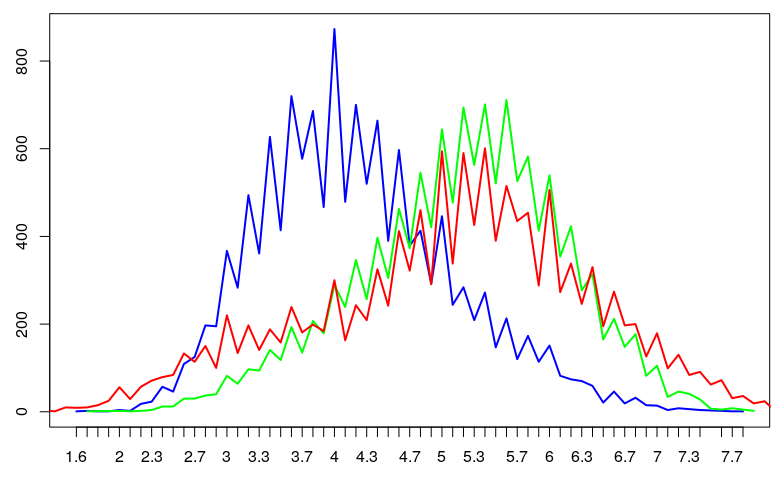
\includegraphics[scale=0.4]{graphs/lexiconDist.png}
\caption{Frequency of words over each dimension in bag-of-words dataset R: Valence, B: Arousal, G: Dominance. The dataset ranks the words on a scale between 0 and 10, which is adjusted for use with the EmoBank dataset}
\label{lexiconGraph}
\end{figure}

As we can see from Figure \ref{lexiconGraph} there is a bias in the data for each dimension, and the average value for the Arousal dimension is noticeably lower than the other two. Whether this affects the suitability of this dataset for use in building a prediction model will be explored further.

\subsection{EmoBank}
This dataset is the most important one for this project, as it contains 10,000 English sentences covering multiple genres, all annotated with their own VAD values \cite{emoBank}.

This dataset contains values for each sample sentence from both the writer and the reader of the text, but due to the findings in the paper accompanying it \cite{emoBank}, only the values given by the reader will be used, as it concluded that this perspective has higher emotionality and therefore they should be easier to build a more accurate model with.

Many existing sentiment analysis tools train over very large datasets, scraping information from things such as movie reviews \cite{socher2013recursive} or from Tweets \cite{towardsDS}, and so usually have above 100,000 samples to train from. In this case, the EmoBank dataset only contains 10,000 sentences, and whether this is a setback will have to be taken into account. These larger datasets could not be used in this case since they are not annotated in a way that allows a more complex emotion to be calculated, since they are usually only scored by their Valence values. 

We can see from Figure \ref{dist:vad} that most of the EmoBank data lies in the middle of the dataset, meaning that there is an imbalance in data. This can cause issues for building a prediction model from, as many prediction models will overfit on the majority class or range of values, predicting the most likely values every time. Dealing with this to be able to use the Emobank dataset the most effectively will also be explored further.

\begin{figure}[h]
\centering
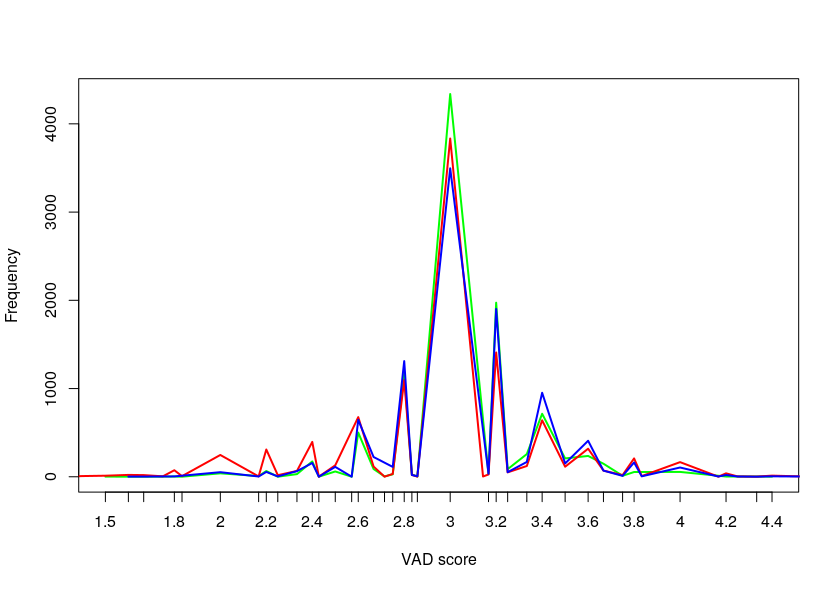
\includegraphics[scale=0.5]{graphs/VADdistribution.png}
\caption{Graph showing data distribution over the Emobank Dataset. R: Valence, B: Arousal, G: Dominance}
\label{dist:vad}
\end{figure}

 
   
\section{Methodology}
\subsection{Data Imbalance}

The initial issue faced was how to split the continuous variables supplied by the EmoBank dataset into discrete categories.

An initial look at the data shows that there is a large number of sentences represented with valence values in the neutral, and very few representing the extreme cases. 

\todo{LINE GRAPH WITH NUMBER OF SAMPLES}

The simplest way to initially categorise the data is to round to the nearest whole number, but as shown in figure \ref{dist:5cat}, the extreme classes are not well represented, and would prove very difficult to train a model off since there is such little data there to provide insight. Also having 5 discrete classes for each dimension provides more detail than is necessary for the task at hand.


\begin{figure}[h]
\caption{Graph showing data distribution when split into five classes}
\centering
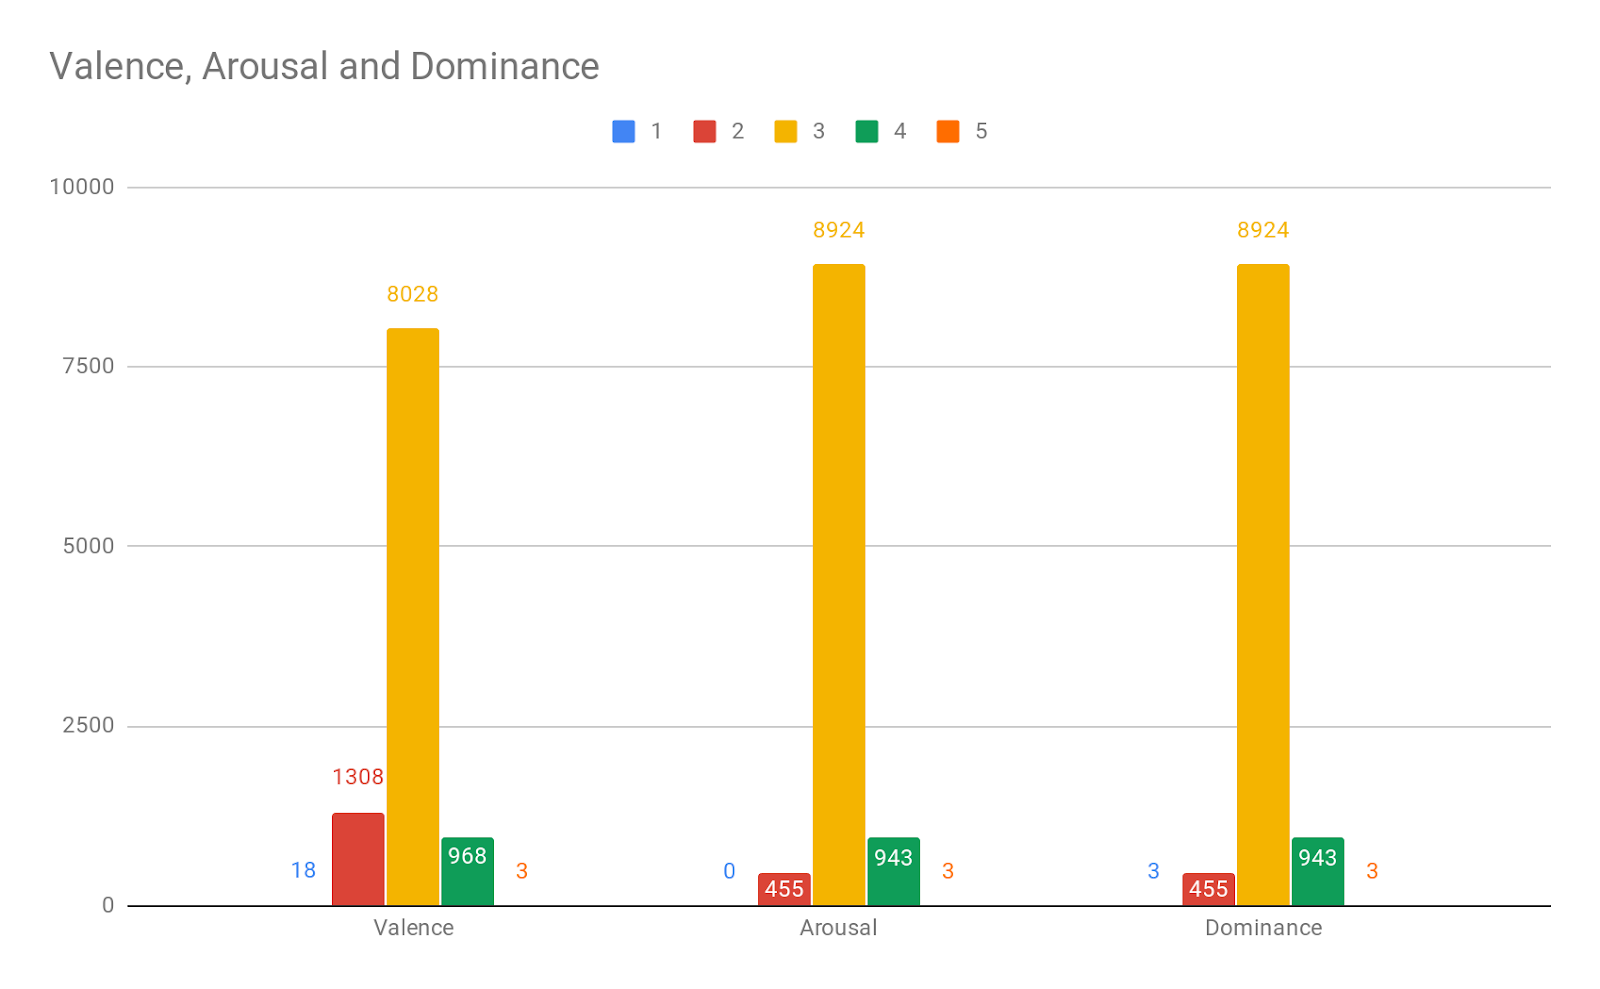
\includegraphics[scale=0.3]{graphs/5catDist.png}
\label{dist:5cat}
\end{figure}

Splitting each dimension up into positive or negative values, splitting each sentence into whether it is above or below 2.5 also is an option, allowing easier analysis to compare to other work which generally does just split the valence into positive or negative. The issue here is that the data imbalance is still very great, particularly with the Arousal and Dominance dimensions.

\begin{figure}[h]
\caption{Graph showing data distribution when split into binary positive and negative classes}
\centering
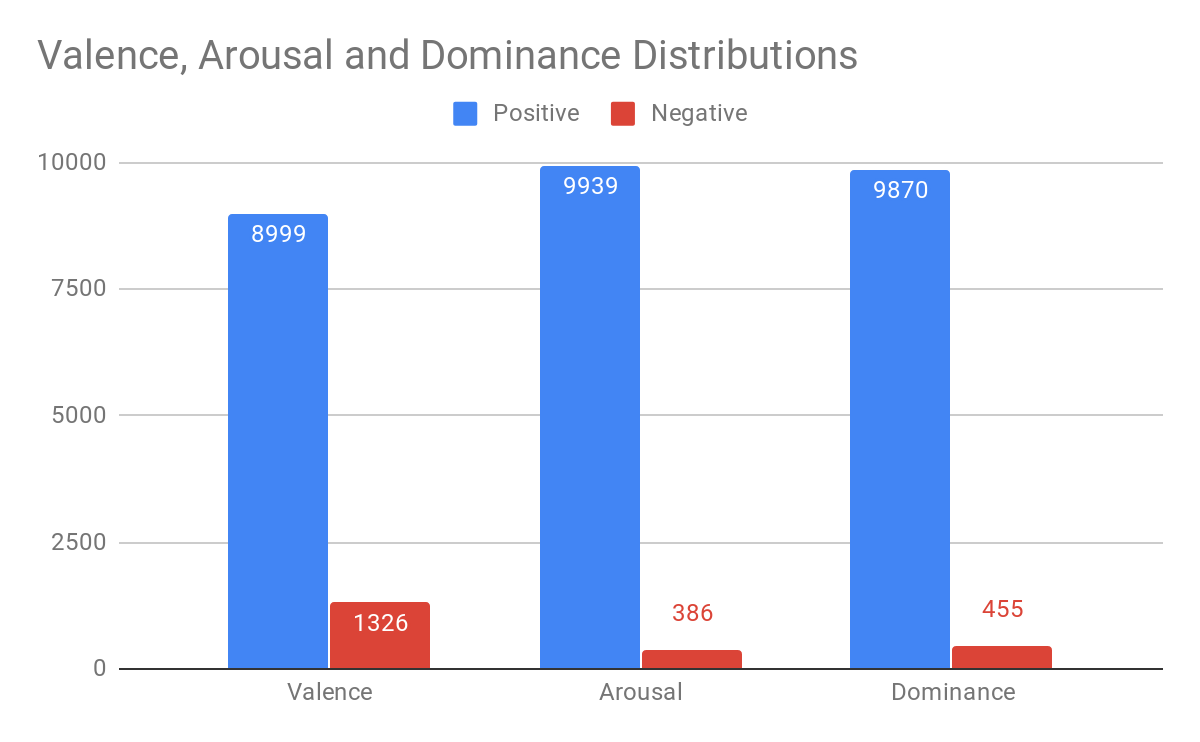
\includegraphics[scale=0.3]{graphs/binaryDist.png}
\end{figure}

A middle ground can be found when splitting the data into positive, neutral and negative classes, as even though there is still a data imbalance there, it is less severe, and so is used for the rest of analysis over the data.

\begin{figure}[h]
\caption{Graph showing data distribution when split into positive, neutral negative classes}
\centering
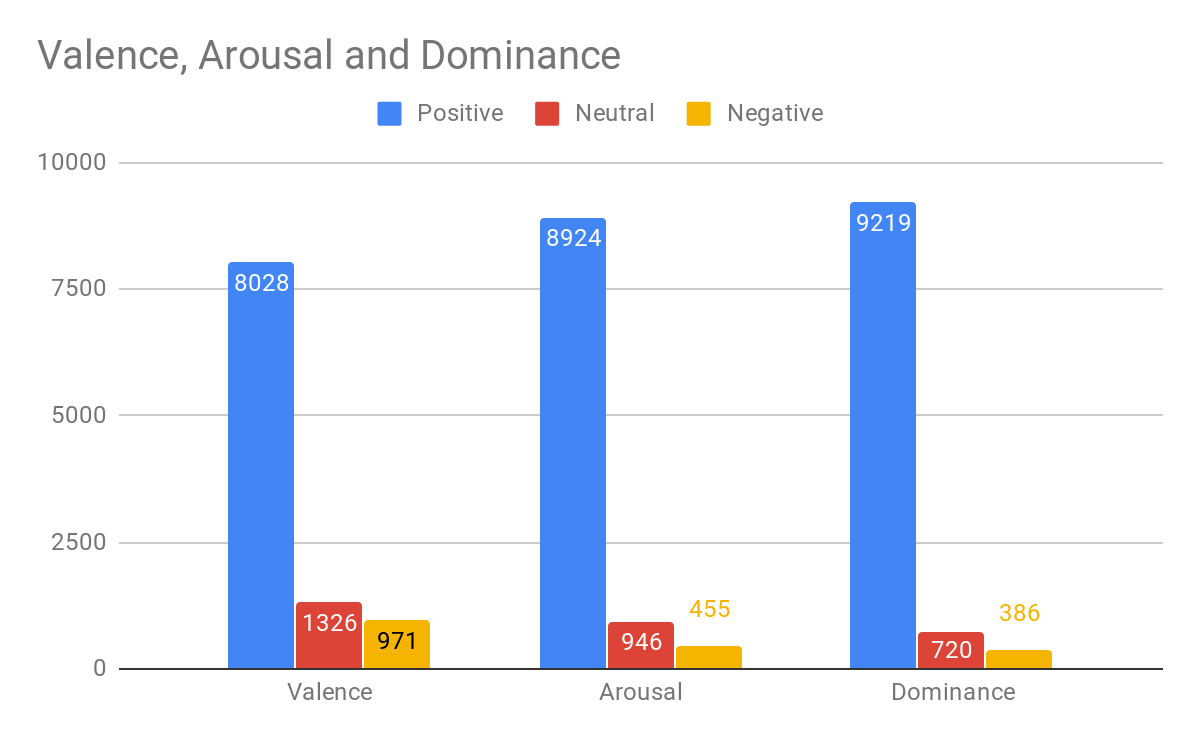
\includegraphics[scale=0.3]{graphs/nonBinaryDist.png}
\end{figure}


\subsection{Hypothesis Tests}


To argue for each of the decisions made when building the final model, a hypothesis test with a 90\% confidence level will be carried out.

Due to the imbalance in the data, a prediction accuracy cannot be used for comparing the models. This is because the majority class dominates, with it being the most likely to be predicted as there are simply more examples available. \cite{al2015applied} 

The F1 score of the prediction model is used in the hypothesis tests. The F1 score is the weighted average of the Precision and Recall of a model, which are defined as follows: 

$$ F1 = 2 * \frac{Precision * Recall}{Precision + Recall} $$

For each investigation that is carried out, a confusion matrix is be produced so that the precision and recall values for each result can be calculated, which will have the following structure: 

\begin{center}
\begin{tabular}{ |p{3cm}|p{3cm}|p{3cm}|p{3cm}|p{3cm}| }
 \hline
  & \multicolumn{3}{|c|}{Predicted} &\\
 \hline
   Actual & Negative & Neutral & Positive &\\
    \hline
    Negative &  True Negative   &  False Negative  & False Negative & Total Negative\\
    Neutral & False Neutral & True Neutral&  False Neutral & Total Neutral \\
    Positive & False Positive & False Positive &  True Positive & Total Positive\\
    \hline
    & Total Predicted Negative & Total Predicted Neutral & Total Predicted Positive & \\
 \hline
\end{tabular}

\end{center}

And then the precision and recall values can be calculated as follows:

$$ Precision_{Class} = \frac{True Class}{Total Predicted Class} $$

$$ Recall_{Class} = \frac{True Class}{Total Class} $$



The hypothesis test that will be performed on the data will be the Wilcoxon Signed-Rank Test, since the comparison between the data will be on two related samples, looking for differences in their population rank means, and the data cannot be assumed to be normally distributed, meaning that this is the best test to be using in this case. \cite{wilcoxon1970critical}


Each of the experiments are run with stratified k fold validation, with the data from each fold being used for test comparisons, with k set to 10. The folds are stratified so that the representation of each class remains the same in each fold which is needed due to the large data imbalance. \cite{kohavi1995study}


\subsection{Lexicon Analysis}
\todo{do this}


\subsection{Data Pre-processing (N-Gram and Feature selection)}

Following Ricky Kim's investigations into semantic analysis \cite{towardsDS}, an investigation into optimising the format for the data input is carried out. 

To be able to analyse the text, the sklearn CountVectorizer library is used to return a sparse matrix of the counts of each word in the input vocabulary. \cite{sklearn}

From this we can limit the number of features that we can take, here the number of features is the number of most popular N-Grams, and we can set the N-Gram range easily. 

The previous investigation only tried N-Gram values ranging up to trigram, but to ensure that this is an optimal result, the experiment will be carried out up to fourgram.

The range of features that was used previously was up to 10,0000 number of features because the results did not improve after this, but since we are using a different dataset, the number of features tested was increased until the resultant graph implied that the F1 score did not improve further. 

The model used to investigate how the F1 score varies as the inputs change will be a Logistic Regression model, as this is the most commonly used one \todo{cite}

\begin{figure}[h]
\caption{Experimental Results for varying the number of features and values for N-Gram sequences}
\centering
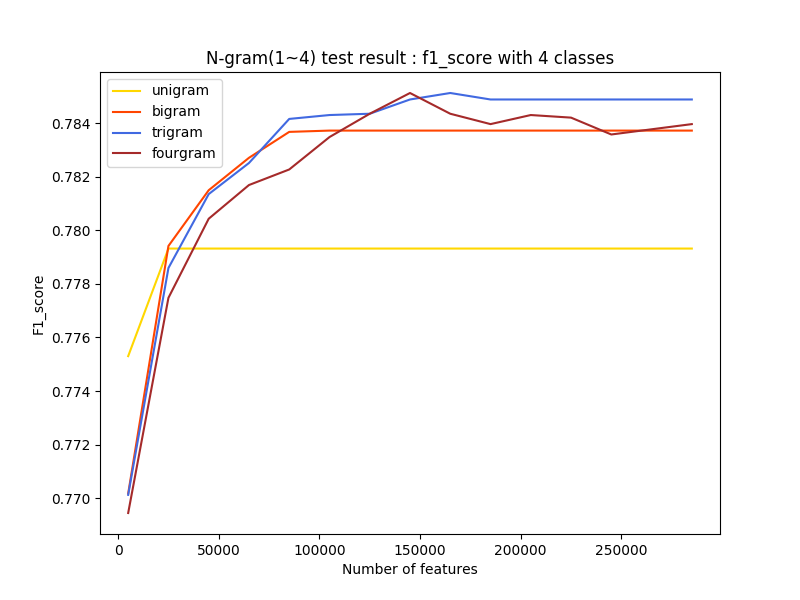
\includegraphics[scale=0.7]{graphs/nGramBinaryGraph300000.png}
\label{ngramGraph}
\end{figure}

As shown in Figure \ref{ngramGraph}, the F1 score improves as the N-Gram value increases up to a point, and also increases as the number of features also does. An explanation of why the values for fourgram are generally less than for trigram could be because the dataset is not that large and therefore predictions are less accurate since the relationships between the words cannot be properly established, so for our purposes we can leave out fourgram as it requires \todo{x much more processing power than trigram}.

As we want do not want to use unnecessary processing power, we want the number of features in the training set to be as low as possible. 

Using the trigram values to compare, the hypothesis test shows that the F1 score still increases after 85,000 features as shown below:

$$ H_0:  \textnormal{F1 score at 85,000 features is the same than at 165,000 features (the peak on the graph)}$$

$$ H_a: \textnormal{F1 score at 85,000 features is less than at 165,000 features} $$

Using the Wilcoxon rank sum test with 90\% confidence interval 
p = 0.08 so reject $H_0$

But the score for F1 does not increase significantly after 105,000, which is shown as follows:

$$H_0: \textnormal{F1 score at 105,000 features is the same than at 165,000 features} $$
$$H_a: \textnormal{F1 score at 105,000 features is less than at 165,000 features}$$

Using the Wilcoxon rank sum test with 90\% confidence interval 
p = 0.15 so reject $H_a$


We can conclude that the optimal number of features to use in the model is 105,000, and this value will be used in the rest of the investigations as to maximise the score of the result model.



Using this value to compare bigram and trigram results with the following test 

$$ H_0: \textnormal{F1 score of Bigram and Trigram is the same at 105,000 features} $$
$$ H_1: \textnormal{F1 score of Bigram is less than Trigram at 105,000 features} $$

Using the Wilcoxon rank sum test with 90\% confidence interval 
p = 0.10

This value is just on the margin, but we will take it as enough evidence that trigram gives a higher F1 score, so can conclude that the value for N in the N-Gram selection will be tri-gram. The R scripts for running these tests are referenced in Appendix
\todo{make a file}
\ref{appendix:hypothesis}.

\pagebreak

\subsection{Model Selection}

To choose the models to compare, we will take the top models compared in previous sentiment analysis work \cite{towardsDS} and see which can work best in this situation.

\begin{figure}[h]
\caption{Graph showing the different F1 scores for varying types of classifier}
\centering
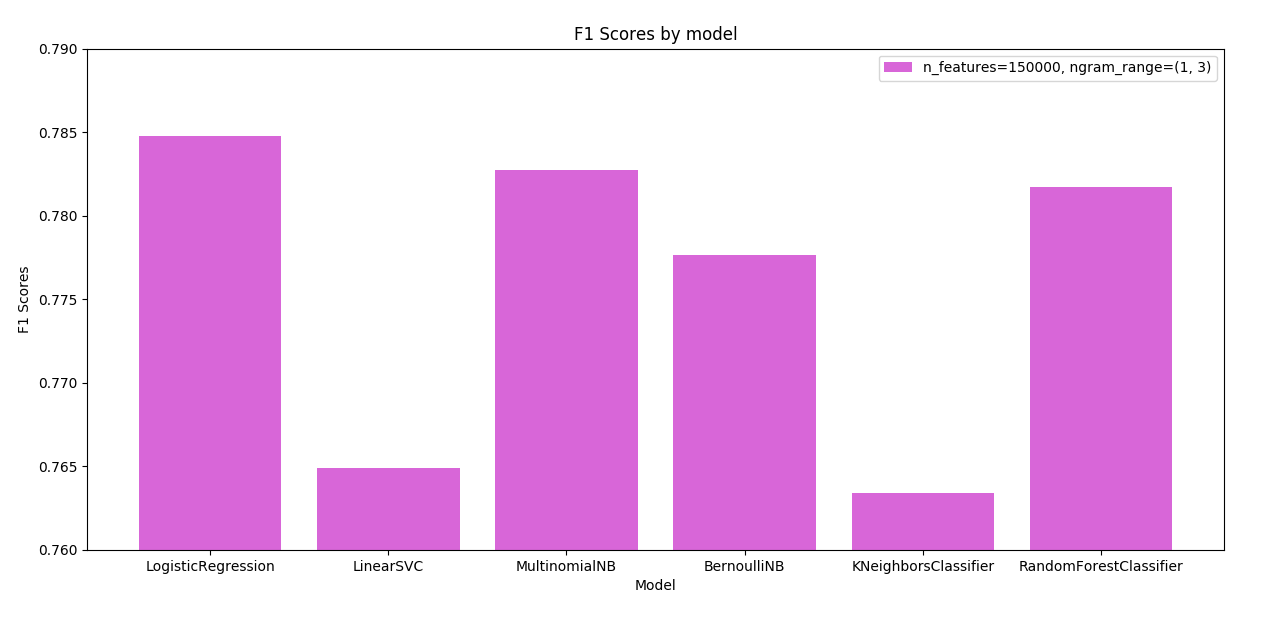
\includegraphics[scale=0.5]{graphs/models.png}
\label{model:graph}
\end{figure}


The inbuilt models in the sklearn package with default settings were used for initial comparison, and as we can see from Figure \ref{model:graph} the difference between the models is very slight, with the F1 scores all within a 3\% range. As expected logistic regression leads to the highest results, but to be certain we run a hypothesis test to ensure the F1 score is greater than the next highest result, Multinomial Naive Bayes as follows:

$$ H_0: \textnormal{F1 score for the Logistic Regression is the same as Multinomial NB}$$
$$ H_a: \textnormal{F1 score for the Logistic Regression is the greater than Multinomial NB}$$

Using the Wilcoxon rank sum test with 90\% confidence interval, p = 0.02 so reject $H_0$, so we can select Logistic Regression as the optimal classification model to use.


\subsection{Oversampling and Undersampling}

To carry out the investigation of applying the oversampling and undersampling methods, the library functions in the imblearn API is used, which can be used in conjunction with the sklearn methods easily. 

Since it is unclear whether these methods will actually improve the model, comparing against the model that we already have is necessary, and as we can see from Figure \ref{oversamplegraph}, using any oversampling methods actually decreases the F1 score by a significant amount. 


\begin{figure}[ht]
\caption{oversample}
\centering
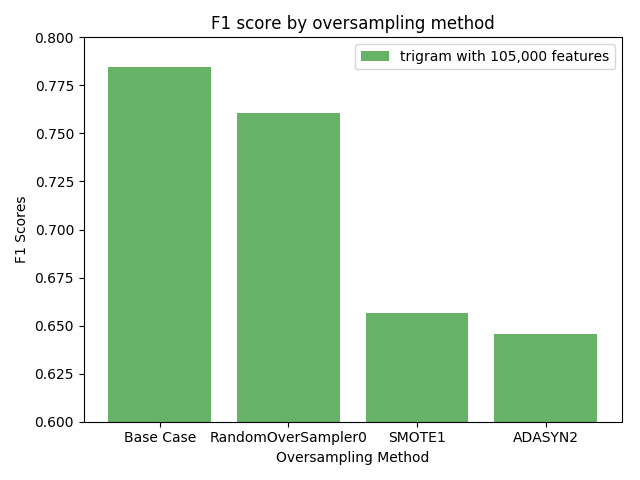
\includegraphics[scale=0.7]{graphs/oversampling.png}
\label{oversamplegraph}
\end{figure}

An explanation as to why this is happening is most likely a combination of using textual data, which is known to cause issues with oversampling methods, and the severity of the imbalance in the data. In the valence class, which is the one we are analysing at this point, the negative samples make up less than 10\% of the overall data and therefore many of the synthetic samples that are created will not make grammatical sense and be of poor quality. 


The undersampling methods were known to not give promising results, but due to the issues with oversampling over such imbalance, briefly investigating this was something that could potentially have worked, but as shown in Figure \ref{undersamplegraph}, they all made the model perform significantly worse and hence can be disregarded.

\begin{figure}[ht]
\caption{undersample}
\centering
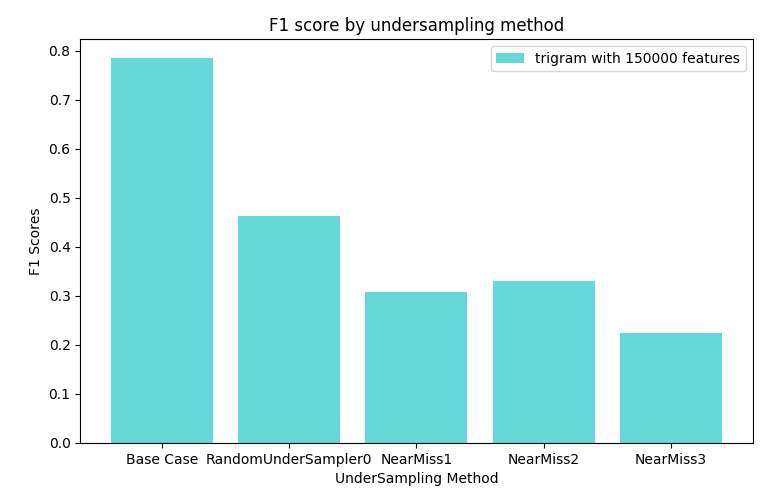
\includegraphics[scale=0.7]{graphs/undersample.png}
\label{undersamplegraph}
\end{figure}

\pagebreak

\subsection{Final Model}

The final model that was produced then had the following characteristics: 

\begin{itemize}
    \item The data was formatted into trigram tokens.
    \item The most frequent 105,000 n-gram tokens were used as input features.
    \item The classification model is Logistic Regression.
    \item No oversampling or undersampling techniques were applied.
\end{itemize}

Which results in a model that has an average F1 score of 0.7843 (4 significant figures). 

\subsection{Implementation}

The simplest solution to provide an interface between the final produced semantic prediction model and the Spotify API is to create a web application. The final classification model was hosted on a very simple python server that takes text as an input, and returns whether it classes the text as Positive, Negative or Neutral for each Valence, Arousal or Dominance dimension. 

The final solution, as shown in Figure \ref{implementationLayout} consists of three distinct hosted solutions, two of which access the API hosted by Spotify to access song data and authentication.

The UI was chosen to be built in Angular.js and the music API with Node.js due to prior development knowledge, and hence ease of prototyping. 
To ensure that any resultant song given back was one that the user could relate to, the song that is given back is taken from the users recent top songs. 
The music API, built in Node.js is influenced by the structure of existing Spotify API projects \cite{moodtape}, is built mostly using the Node Package spotify-web-api-node \cite{nodeSpotify} which allows for ease of dealing with authenticating users, so that the users top songs can be accessed.

\begin{figure}[ht]
\caption{General layout of how the web application is structured.}
\centering
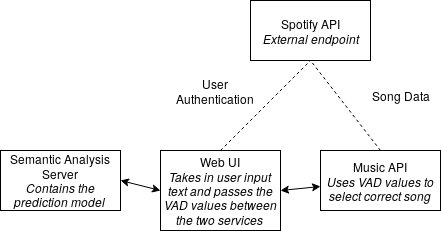
\includegraphics[scale=0.6]{litImgs/interfaceLayout.png}
\label{implementationLayout}
\end{figure}
                

Choosing how to relate the VAD values to the data returned by the Spotify was relatively arbitrary, and something that if there was more time could be investigated further. Since the song data returns a Valence value for the song, that is an easy relation, and it was chosen to map the Arousal to the "Energy" attribute, and the Dominance to the "Danceability", but this is something that can be improved upon as plenty of other data is also returned about the song which can be related to the three dimensions, such as relating the tempo and loudness of the songs.

The main goal of the implementation is to attempt to relate an emotion which is subjective, to a song since that is also subjective so a decision was made to not show the user the VAD values, and just the result song to begin with. After the users reaction to the response song has been assessed, the calculated Ekmans emotion can be shown (calculated by the figures given in Table \ref{ekmansTable}) and discussed.

\begin{figure}[ht]
\caption{Layout of main UI page}
\centering
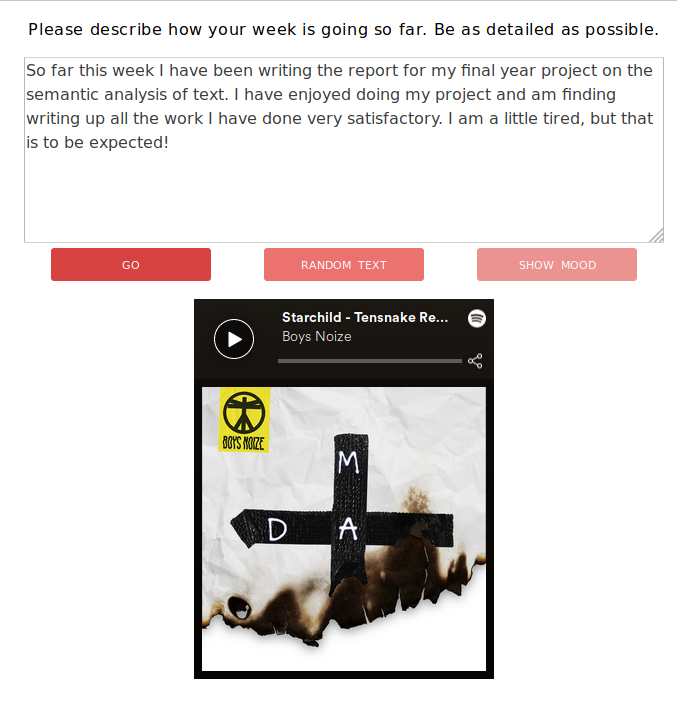
\includegraphics[scale=0.4]{litImgs/UIScreenshot.png}
\label{UIlayout}
\end{figure}

\begin{figure}[ht]
\caption{User activity through the application}
\centering
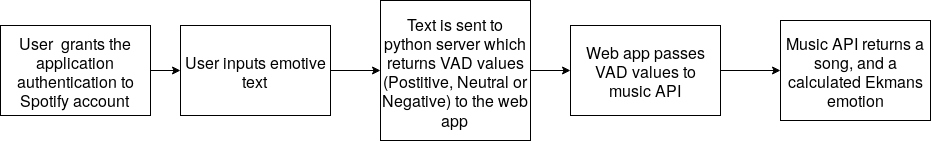
\includegraphics[scale=0.6]{litImgs/interfaceFlow.png}
\label{implementationLayout}
\end{figure}

\section{Results and Discussion}
\begin{itemize}
    \item How can textual sentiment prediction be optimised?
    \item Does using more than 1 dimension to classify emotions provide more insight, and how can this be quantified?
\end{itemize}

\section{Conclusion}

From a personal perspective this project has been thoroughly enjoyable. I had almost no machine learning knowledge before starting, and I have learned more than I had anticipated. Being able to apply new techniques to tools that I was already familiar with has been has been an accomplishment, and I am happy with the final product that has been produced. 

Things that I would do differently now would be to formalise the research questions at an earlier point so that less time was spent exploring things which ended up being unnecessary. I'd have also liked to have spent more time getting to know the data, so that the dependency between the classes could have been investigated further. 

Keeping the VAD values in their original continuous form is also something that would be interesting to explore, and comparing results formed from an investigation into this, to the model used in this project would offer more insight into how the Emobank dataset can be utilised.

Exploring ways in which an emotion can be represented, and using them to the greatest effect has been explored in this project. Future investigation of sentiment representation and analysis can be done with a better understanding by using what has been set out in this report, and more work can be done to attempt to quantify something as seemingly unquantifiable as a human emotion.

\pagebreak

\section{Appendix}


\bibliographystyle{unsrtnat}
\bibliography{ref,lit}


\end{document}
